\documentclass[a4paper,10pt,conference]{ieeeconf}

\IEEEoverridecommandlockouts
\overrideIEEEmargins
\usepackage{graphics} % for pdf, bitmapped graphics files
\usepackage{epsfig} % for postscript graphics files
\usepackage{mathptmx} % assumes new font selection scheme installed
\usepackage{times} % assumes new font selection scheme installed
\usepackage{amsmath} % assumes amsmath package installed
\usepackage{amssymb}  % assumes amsmath package installed
\usepackage{multirow}

\title{\LARGE \bf
Joint Visual and Motor Learning for Object Modeling and Recognition
} 

\author{B. Caputo, T. Tommasi, C. Castellini, N. Noceti, F. Odone, G. Sandini%
\thanks{This work is  supported by the EU Integrated Project project DIRAC (IST-027787, BC and TT) and by the
project Contact (NEST 5010, CC).}%
\thanks{B. Caputo and T. Tommasi are with the Idiap Research Institute,
        {\tt\small bcaputo@idiap.ch, ttommasi@idiap.ch}}%
\thanks{C. Castellini is with the LIRA-Lab, University of Genova, Italy, and the
        DLR --- German Aerospace Research Center, Wessling, Germany,
        {\tt\small claudio.castellini@unige.it}}%
\thanks{G. Sandini is with the Italian Institute of Technology, Genova, Italy,
        {\tt\small giulio.sandini@iit.it}}%
\thanks{N. Noceti and F. Odone are with the Computer Science Department of the University of Genova, Italy,
{\tt\small odone@disi.unige.it, noceti@disi.unige.it}}%
}
\DeclareMathOperator*{\argmax}{argmax}

\begin{document}

\maketitle
\thispagestyle{empty}
\pagestyle{empty}

\begin{abstract}
  Grasping is one of the most challenging tasks in advanced robotics...

\end{abstract}

\section{Introduction}
\label{sec::introduction}
Consider Figure \ref{fig:chairs}, representing $(a)$ a chair, and $(b)$ Santiago
Calatrava's ``sedia redonda'', the round chair, a particularly stylish object of
design sold as a chair in the Sixties. What makes us claim that these objects
both belong to the category of chairs? Indeed, this is an ominous problem in
object recognition: too often the category of an object is determined by its
function rather than by its visual appearance alone. The very concept of object
has been re-defined by Gibson \cite{gibson} in terms of its affordances ---
``what one can do with it''. According to this view, what ties both the objects in
Figure \ref{fig:chairs} to the category of chairs is the fact that they are
used to sit down.

Further hints at a strong link between perception and action come from neuroscience,
in particular from the mirror neurons paradigm \cite{fadiga}. According to the
mirror theory, neural correlates are found for both the performance of a grasping
action (mainly involving the sensorimotor system of primates) and its visual
representation when performed by another primate (involving the visual system only).
If this is true, as it seems, then the monkeys' (and our) object classification is
so robust mainly because these biological systems \emph{know what to do} with the
objects they see --- a capability which machines lack, so far. Picture, for instance,
how much easier automated object recognition of a mug would be under changing illumination
conditions, if only our machine had an idea of how to grasp something which looked like
a mug.

Inspired by these considerations, we hereby define a theoretical framework for
reconstructing \emph{active} sensory modalities from \emph{passive} ones, that is in
short, for figuring out what to do with what one sees, hears, smells etc. In particular,
we enforce one such schema using a multi-variate regression technique to associate
\emph{object visual features} to related \emph{human grasping postures}. This schema is
called a \emph{Visuo-Motor Map} (VMM) and is trained
using a large database of visual and motor data collected from human subjects, that
we call the \emph{Visuo-Motor Grasping dataBase} (VMGdB). The immediate result is the
ability of retrieving a (set of) grasping posture(s) just by seeing an object; this
ability, which we call \emph{grasp priming}, has obvious applications in robotic fields
where (semi)autonomous grasping / fine manipulation is reuquired, such as robotic surgery,
humanoid robotics, teleoperation, advanced hand prosthetics etc.

Since, though, the focus of this work is on enhancing object reocgnition, we then show
that these grasping postures, reconstructed by the VMM, dramatically improve the
classification rate of a standard object classifier.

The paper is organised like this: in Section \ref{sec::framework} we define the general
multi-modal learning framework, and then we describe the instance under examination;
we then describe in detail the vision-related unit (Section \ref{sec::vision}) and the
regression schema employed to build the VMM (Section \ref{sec::regression}). We then show our
experimental results (Section \ref{sec::experiments}) and conclude in Section \ref{sec::concl}.

%\begin{itemize}
%
%\item learning by imitation great capability of cognitive systems. It permits to learn how to grasp a cup never seen before just by seeing someone else doing it.
%Fundamental learning mechanism etc 
%
%\item a widely accredited hip is that the underlying mechanism of learning by imitation is the existence of a sensor motor map that links
%the visual perception of an object to the motir position of the hand when it manipulates it. Mirror neurons blabla 
%
%\item another consequence of the existence of a sensor-motor map is that when we learn an object by seeing and manipulating it, we are then able
%to recognize it with a higher degree of accuracy and robustness than if we would have learned it on visual data only. 
%
%\item Enabling a robot to display similar abilities is one of the holy grails of research in artificial cognitive systems. 
%
%\item In this paper we present a mirror neurons inspired algorithm for building perception action maps between visual, passive perception and motor, active
%perception. During learning, the algorithm takes as input visual and sensomotor data and (a) it builds a mapping between the two modalities (b) it builds 
%a classifier on both modalities. After training, wehn presented with a visual input, the system is able to perform grasp priming (= is able to predict
%which are the possible way to grasp the seen object; this information could be used to pre-activate a robot hand) and enhanced visual recognition
%(= is able to recognize objects with a higher degree of accuracy and robustness compared to a model learned only on visual features, even if
%the sensor modality is not perceived by the agent). Experiments show that.....
%
%\item in the rest of the paper...
%
%\end{itemize}

\subsection{Related work}
The capability to recognise and categorise objects is a crucial
ability for an autonomous agent; and in robotics, it is inextricably
woven with the ability of grasping an object. In cognitive science, the
theoretical link between vision and manipulation was provided by 
Gibson, according to whom an object is characterized by three
properties: (1) it has a certain minimal and maximal size related to the
body of an agent, (2) it shows temporal stability, and (3) it is manipulable
by the agent. These properties imply that the object is defined in relation
to an embodied agent able to manipulate the object. Therefore the set of
possible manipulation actions are a crucial part of the object definition
itself. 

Interestingly, the theory of affordances has recently found neurological evidence,
it is claimed, in the mirror neurons paradigm \cite{gallese-96,rizzolatti-04}.
According to it, structures exist in the high primates' brain which will fire
if, and only if, an object is grasped (which mainly involves the sensorimotor
system) or is seen grasped by an external agent (involving the visual system only,
\cite{umilta-01}). In addition to the original findings in monkeys, very recent
evidence has been produced for the existence of such structures in humans
\cite{friston09}. If this is true, then the human object classification is
so robust exactly because we \emph{know what to do} with the
objects we see --- a capability which machines lack, so far.

This idea has so far been little exploited; among the positive cases there
are \cite{metta-06,lopes-05} who take an exquisitely robotic perspective,
letting their systems acquire motor information about objects by
having a humanoid robot actually manipulating them. On the other hand,
the vast majority of work on object recognition and categorization
models objects starting from static images, without taking into account
their 3D structure and their manipulability \cite{griffin_perona_cvpr2008,leibe_etal_ijcv2008}.
Few very recent attempts try to capture the Gibson's view. The approach
proposed in \cite{gupta_davis_cvpr2008} presents a Bayesian framework that
unifies the inference processes involved in object categorization and
localization, action understanding and perception of object reaction.
The joint recognition of objects and actions is based on shape and motion,
and the models take as input video data. In \cite{kjellstrom_etal_eccv2008},
the authors consider objects as contextual information for recognizing
manipulation actions and vice versa. The action-object dependence is
modelled with a factorial conditional random field with a hierarchical
structure. In both approaches, objects and their affordances are first
modelled separately, and combined together in a second step. This does
not consider the embodiment of the agent manipulating the objects.


\section{The Visuo-Motor Grasping Database}
\label{sec:database}
\begin{figure*}[tb]
	\centering
	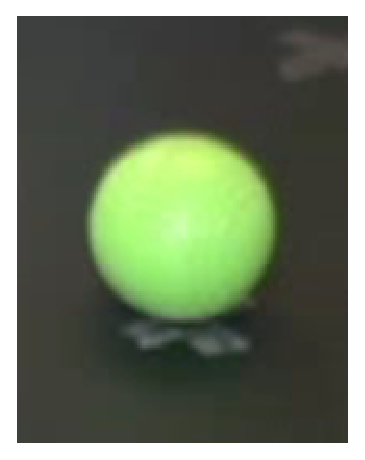
\includegraphics[height=1.75cm]{images/objects/palla}
	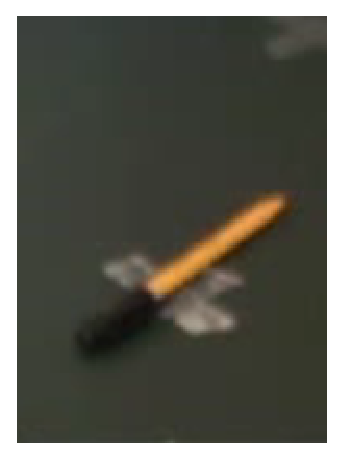
\includegraphics[height=1.75cm]{images/objects/penna}
	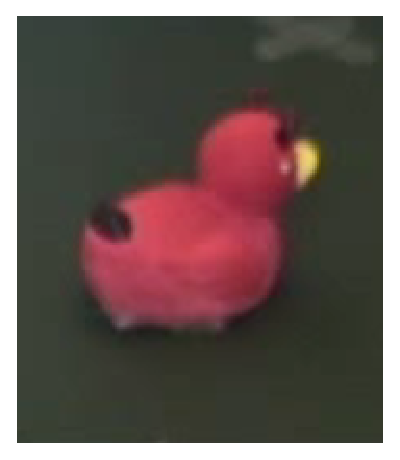
\includegraphics[height=1.75cm]{images/objects/papera}
	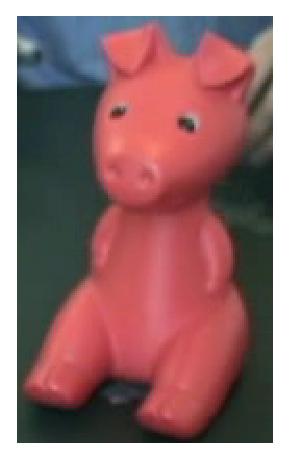
\includegraphics[height=1.75cm]{images/objects/porcellino}
	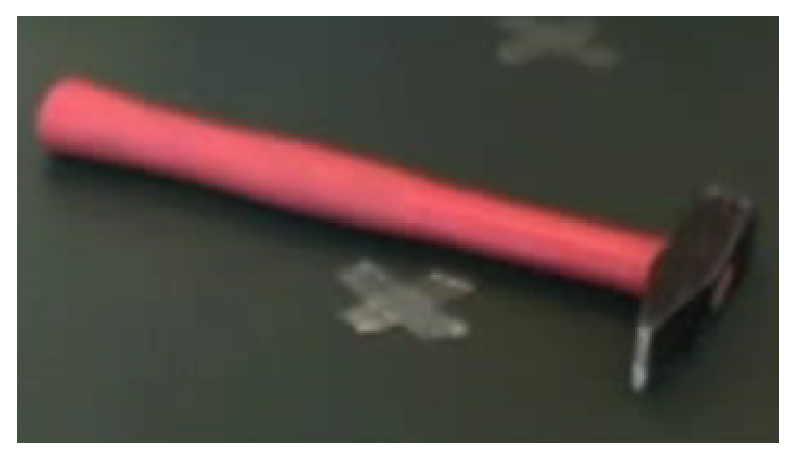
\includegraphics[height=1.75cm]{images/objects/martello}
	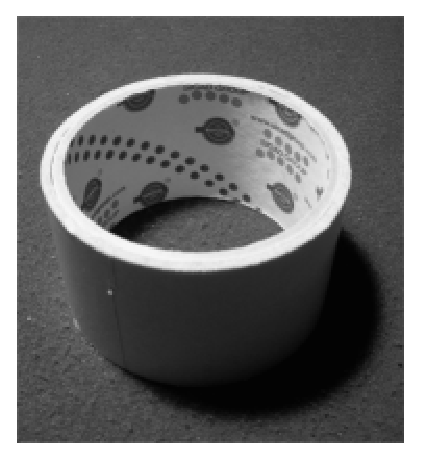
\includegraphics[height=1.75cm]{images/objects/scotch}
	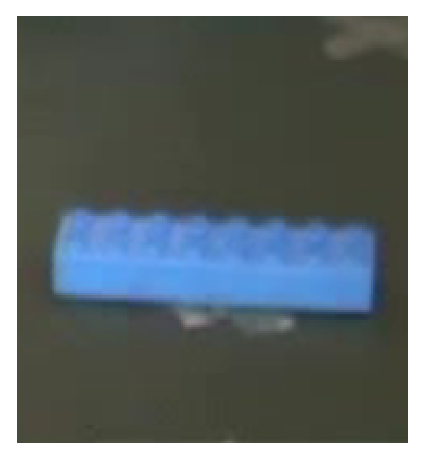
\includegraphics[height=1.75cm]{images/objects/lego}\\
	\vskip 0.1cm
	\includegraphics[width=0.12\textwidth]{images/objects/cylinder}
	\includegraphics[width=0.12\textwidth]{images/objects/flat}
	\includegraphics[width=0.12\textwidth]{images/objects/pinch}
	\includegraphics[width=0.12\textwidth]{images/objects/spherical}
	\includegraphics[width=0.12\textwidth]{images/objects/tripodal}
	\caption{Top row: the objects used in our experiments. Bottom, the grasp types we consider: \emph{(left to right)} cylindric power grasp, flat grasp, pinch grip, spherical and
	tripodal grip.}
	\label{fig::grasps}
\end{figure*}

The VMGdB dataset is built considering 7 different objects ((see Fig. \ref{fig::grasps}), top) and 5 grasps ((see Fig. \ref{fig::grasps}), bottom).
 20 different actors participated to the acquisition, during which  
 each object was grasped in one or more  ways, according to the many-to-many relationship reported in Table \ref{tab:manytomany}. In total
we consider 13 different pairs (grasp,object), and, for each triple {\em (object, grasp, actor)}, we acquired 20 replicates of the grasping experiment.
 
 {\small
\begin{table}
\begin{tabular}{c | c c c c c c c}
& ball & pen & duck & pig & hammer & tape & lego brick \\
\hline \\
cylindr. pow. & & & & X & & & \\
flat & & & &  & X & & X \\
pinch & & X & X & & & X & X \\
spherical & X & & & & & X & \\
tripodal & X & X & X & & & X & 
\end{tabular}
\caption{\label{tab:manytomany} Mapping grasps-objects. Each actor performs grasping actions on 13
object-grasp type pairs.}
\end{table}
}
 
We obtained 5200 experiments {\em (object, grasp, actor, expnum)}, and for each of them the VMGdB stores the following information:
\begin{itemize}
\item {\bf Visual information.} 2 video sequences  acquired by 2 color cameras with different focus -- one is the object, the other one is the grasping action. The video sequences
are associated to 2 data files reporting the video frames time-stamps, allowing for synchronization with the sensor data;
\item {\bf Hand posture sensor information.} 1 data file containing the hand posture sensor data acquired by a CyberGlove
\cite{cyberglove}. 
For each posture the glove returns $22$ $8$-bit numbers linearly related to the angles of the actor's hand joints. 
The sensors describe the position of the three phalanxes of each finger (for the thumb, rotation and two phalanxes), the four finger-to-finger
abductions, the palm arch, the wrist pitch and the wrist yaw. Again, the sensor data are associated to acquisition time-stamps for synchronization. 
\end{itemize}


\section{Theoretical framework}
\label{sec::framework}
\section{A theoretical framework for multi-modal learning}
\label{sec::framework}

As outlined in the Introduction, we assume that there exists a mapping between (sets of) patterns belonging to different modalities --- here we focus upon the relations which exist between a passive and an active modality. In the aforementioned example dealing with objects (as seen) and grasping them, something like what is shown in Figure \ref{fig::implementation} is sought for.

\begin{figure}[h!]
	\centering
	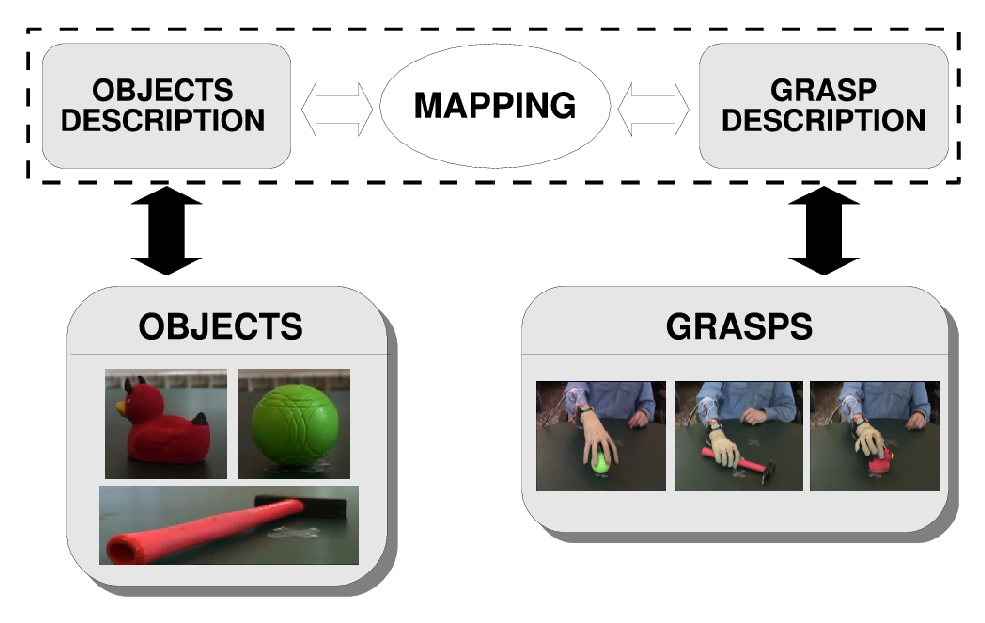
\includegraphics[width=0.7\textwidth]{images/schema_implementazione}
	\caption{An instance of the framework we propose: estimating a
     mapping between appropriate visual descriptions of objects and
     classes of grasp actions. For the time being, we assume that such
     relation is a one-to-one mapping.}
	\label{fig::implementation}
\end{figure}
%\vskip -0.5cm

In general, active modalities are not available to a biological system during the prediction phase, but only during the training phase. A paradigmatic example is that of a human infant learning how to grasp an object: by repeatedly trying to apply, e.g., a cylindric grasp to a bottle, he will learn not only to do it more and more efficiently, but also that a bottle is better be grasped cylindrically when moving it or bringing it close to the mouth. Later on, the sight of a bottle will remind the young human what one of the correct grasps is for that particular object. 
A \emph{perception-to-action map} (PAM) is the equivalent of such training for a biological system: a model to reconstruct an active modality from a passive one. The PAM of our example is a mapping from visual features of an object to motor features of the grasping action used for that object. In general such a map is many-to-many: both a hammer and a bottle can be grasped cylindrically\footnote{the nomenclature of grasp types loosely follows that of Cutkosky \cite{cutkosky}.}), and as well a mug can be handled either cylindrically or by the handle. In this work we make the simplifying assumption that for a specific object there is just one acceptable grasping action --- the PAM is one-to-one.
A PAM is useful in passive pattern recognition (e.g., classifying an object just by seeing it) since it augments the input space with PAM-reconstructed active patterns (e.g., classifying the same object from its sight \emph{and the associated grasp}). In this preliminary work we focus upon a simpler problem, namely that of checking whether, given the visual features of an object, the PAM-reconstructed grasp is (similar to) the one associated with that particular object. For example, we might train a PAM to reconstruct a pinch grip (hand posture) from the visual features of a pen; given then, in the prediciton phase, the visual features of another pen, will the PAM-reconstructed hand posture of a pinch grip look like a true pinch grip?

% We consider $5$ grasp types, shown in Figure \ref{fig::grasps}, identified by different hand postures.

% \begin{figure}
% 	\centering
% 	\includegraphics[width=0.19\textwidth]{images/cylinder}
% 	\includegraphics[width=0.19\textwidth]{images/flat}
% 	\includegraphics[width=0.19\textwidth]{images/pinch}
% 	\includegraphics[width=0.19\textwidth]{images/spherical}
% 	\includegraphics[width=0.19\textwidth]{images/tripodal}
% 	\caption{The grasp types considered in this work: \emph{(left to right)}
% 	   cylindric power grasp, flat grasp, pinch grip, spherical and
% 	   tripodal grip.}
% 	\label{fig::grasps}
% \end{figure}

In particular, what is needed is: $(i)$ a \emph{vision unit} to extract visual features from an image or a series of images, and $(ii)$ a \emph{regression unit}, which will build the PAM.
%Notice that, given our assumption that this PAM is one-to-one, a simple regression method can be used to build it, i.e., we don't have to resort to probabilistic methods such as, e.g., mixture density networks, as it has been done in literature \cite{richmond}.

%Among the various issues and possible applications taking shape from the general schema described so far, the problem we are interested to face can be stated as follows: supposing that it exists a relation between objects and actions, are we able to model it? Our idea is to exploit such relation to obtain joint information about object and action, that is predicting one of them given the other.\\
%\begin{figure}
%	\centering
%	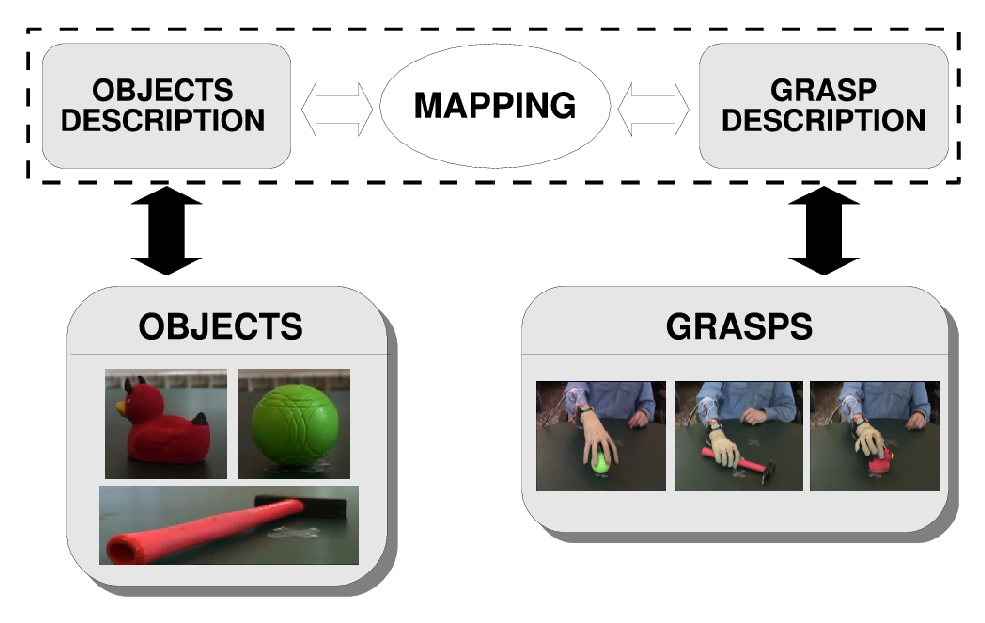
\includegraphics[width=0.7\textwidth]{images/schema_implementazione}
%	\caption{The implementation that we consider relies on estimating a mapping between appropriate descriptions of objects and classes of grasp actions. We assume that such relation is univocally determined by knowing the object.}
%	\label{fig::implementation}
%\end{figure}
%To validate this approach, we implemented a particular instance of the general schema, as shown in Fig.\ref{fig::implementation}, considering grasping actions. From the very general viewpoint we may want to consider classes of objects against classes on grasping actions. However, since our purpose here is to test the pertinence of this procedure, we start instead from the simpler hypothesis that for a specific object there is just one acceptable (class of) grasping action: in other words, we assume that the relation we are looking for can be thought of as a mono-directional mapping.\\
%\begin{figure}
%	\centering
%	\includegraphics[width=0.19\textwidth]{images/cylinder}
%	\includegraphics[width=0.19\textwidth]{images/flat}
%	\includegraphics[width=0.19\textwidth]{images/pinch}
%	\includegraphics[width=0.19\textwidth]{images/spherical}
%	\includegraphics[width=0.19\textwidth]{images/tripodal}
%	\caption{The different grasping types that we consider: from left to rigth, {\it cylinder power}, {\it flat}, {\it pinch}, {\it spherical} and {\it tripodal} grasp.}
%	\label{fig::grasps}
%\end{figure}
%We consider 5 grasp classes, as shown in Fig. \ref{fig::grasps}, ideantified by different fingers poses.
%To summarize, the framework we have in mind should include components able to:
%\begin{itemize}
%	\item model and recognize an object
%	\item extract dynamic (visual and sensorial) information related to the action
%	\item estimate a regression model to obtain information on dynamic actions starting from knowledge about objects appearance.
%\end{itemize}
%This implementation leads us to obtain a system capable of [1] modelling the relation between objects and actions in terms of mapping between appropriate descriptions to handle the multimodality, and [2] predicting the suitable grasping action for a new instance of some known object in the test phase, where motion information are not available. The latter requirement can be thought of as the capability of estimating a {\it virtual grasp}.\\
%The system accepts in input a video signal showing object and dynamic of the action, so a natural choice lies in exploiting low-level measurements extracted from images to capture their appearance. Actions can be further described by means of sensors placed on hand and fingers, allowing to capture peculiarities typical of each grasping.\\
%In the remainder of the paper we will introduce the strategy adopted to implement the system modules and present the preliminary results giving evidence of the pertinence of the proposed approach to solve the problem of interest.

\subsection{Perceptual representations}
\label{sec::vision}
This section describes the visual and motor features used in our framework. We begin with the visual features 
(Section \ref{sec:vis-feat}) and then continue with the motor features (Section \ref{sec:mot-feat}).

\subsubsection{Visual Features}
\label{sec:vis-feat}

% \begin{figure}
% 	\centering
% 	\includegraphics[width=0.5\textwidth]{images/objects/SchemaVisionUnit.pdf}
% 	\caption{A schematic representation of how the visual features are extracted during training(left) and test(right).}
% 	\label{fig::vision}
% \end{figure}

The visual appearance of objects is captured by a dedicated item of the framework, %(see Figure \ref{fig::vision}), 
which
can be sketched as follows.
We first select from the video sequence a set of interesting frames where the object is clearly visible. 
To avoid contamination due to background elements, 
we apply change detection by comparing the selected frames against a background model, and then
restrict our attention on the region of interest (ROI) defined by the object bounding box.
We apply to the ROI a bag-of-keypoints object description \cite{csurka-dance-2004} designed as a two steps procedure \cite{ICIAP}:

\begin{itemize}

\item  We build the global vocabulary, by putting together keypoints extracted from images of all 
the objects into the dataset. As keypoints, we consider a set of randomly sampled points whose 
patch is modeled with a vector valued  descriptor which can be seen as a fixed scale SIFT  \cite{lowe}.
K-means is adopted to cluster the descriptors: the centroids 
(or virtual features) become the words of the visual vocabulary.

\item Both training and test images are thus represented with respect to the vocabulary, with a simple 
nearest neighbor approach.  At the end, visual appearance of objects is summarized with a frequency 
histogram, whose peaks should indicate which virtual features are the most important in modelling a specific object.

\end{itemize}

Notice that the vocabulary size is a system parameter which should be tuned with respect to the complexity of 
objects, to find a trade-off between sparsity of the descriptions and capability of characterizing the objects.           

Finally a remark is in order. From the point of view of appearance-based object recognition, %from visual cues
the experimental scenario is not challenging.
We opted for such a setting in order to keep the focus of the work on the joint modelling of visual and motor inputs.
% being the focus of the work instead to give 
%evidence of the fact that motion actually improves the recognition (classification) performances.

\subsubsection{Motor Features}
\label{sec:mot-feat}
The MPR are simply the $22$ angles returned by the dataglove, considered at
the time of contact of the subject's hand with the object\footnote{A
force-sensing resistor was used to determine the instant of contact.}. The
MPR is therefore a ``snapshot'' of the subject's hand in the instant of
grasping the object.


%\begin{figure}
%	\centering
%	\includegraphics[width=0.5\textwidth]{images/schema_vision.pdf}
%	\caption{A schema of the vision unit. First, suitable frames are extracted from the sequence and objects are located by means of background subtaction (BS). SIFT descriptors of a set of random points are input of a clustering step to get to the final visual vocabulary. Finally, each image is represented with respect to the vocabulary adopting a nearest neighbour (NN) strategy (see text for details).}
%	\label{fig::vision}
%\end{figure}

%As we will discuss in Sec. \ref{sec::experiments}, the system gathers, as one input, a video sequence acting as {\it spectator}, whose focus is on object appearance. The goal of the vision unit is to process the signal to obtain a global model of a set of given objects.
%Figure \ref{fig::vision} shows the pipeline of the vision unit when considering only one object (the same procedure is applied to the whole set of objects). Among the sequence, we first select the frames showing only the object  without any occlusion, then we locate more precisely its position by means of a simple background subtraction. 
%Although in our application there is not an explicit object recognition step, it is clear from the architecture pipeline that a robust and specific object model is functional to subsequent analysis. It is worthwhile also to mention that with the terms {\it object recognition} we indicate the characterization of a specific object instance (againts the concept of categorizing classes of objects).
%We adopt an approach based on local features to describe image structures: because of their popularity a rich variety of local measurements have been proposed in the literature \cite{harris,schmid,lowe} and applied successfully to objects recognition and categorization problems (see \cite{csurka,ferrari} just to name a few). 
%Local approaches tipically include two distinct steps: keypoints extraction and description. 
%However, in our case, a keypoint based-representation often ends up into a poor description
%due to the limited size of the images. We thus built our representation by extracting enough 
%random points  guaranteeing a more homogenous sampling.
%We chose to adopt SIFT descriptors \cite{lowe,schmid2} to model image patches around these points, obtaining a set of {\it words} for each image.\\
%To avoid redundancy and include some global information in our model, we apply k-means \cite{wong}, following the well-known bag-of-words approach \cite{csurka}. 
%We thus build a {\it global} vocabulary, containing SIFT descriptions of all known objects. 
%Image representation is obtained by means of frequency histogram of visual words, selecting for each random point extracted from the image 
%the most similar visual word as nearest neighbor. A normalization step may be advisable for the subsequent data processing.

%\textbf{Questa sezione non mi e' molto chiara....ma la perceptual representation non e'
%fatta da VPR e MPR? Perche' qui descriviamo solo la vision? 
%FEATURES
%---------
%-vision: SIFT, bag of words. 50 words vocabulary, image divided in 4 parts.
%Resulting in feature vectors with 200 elements. 
%-motor: The CyberGlove returns 22 8-bit numbers linearly related to the angles 
%of the subject's hand joints. Resulting in feature vectors with 22 elements.}

\subsection{Learning the Visuo-Motor Map}
\label{sec::regression}
The VMM is supposed to be a regression strategy from visual to motor features, 
as defined above. Since the output is multivariate
(the motor features, consisting of $22$ numbers) and the input is very highly dimensional (the visual features, consisting of $200$
numbers), we decided
to enforce the VMM using neural networks. Each network was kept as
simple as possible: one hidden layer with $20$ neurons,
log-sigmoid transfer function and scaled conjugate gradient 
backpropagation. The training procedure used the early stopping
strategy, i.e. the training set was divided in a new training
and validation set. The network is evaluated on the validation set: 
when the performance stops improving, the algorithm halts. 

Most of these settings are inspired by the work of Richmond and others
\cite{papcun,richmond2007} on audio-to-motor mapping. In fact,
since each object may correspond to several grasps as it happens in reality
(recall the Section above), the relationship between the visual  and the motor features
is highly non-functional and it is in general hard, if not pointless, to
model it using a single NN. Richmond's idea was to model a \emph{probability
distribution} rather than a functional map; here we follow a somewhat more naive approach:
we define an ``archetipal grasp'' related to the specific
object observed. In the case of an object that can be grasped in only one way 
(for instance ``pig''), then the archetipal grasp will correspond 
to it. In case of an object graspable in different ways, then the 
archetipal grasp will correspond to an ``average'' grasp between those 
possible. We expect that this reconstructed grasp will have a 
positive effect on the overall performance of our object recognition system;
at the same time we hope that such representation won't get messed up
with other ones since the output space is also rather high-dimensional.


%The VMM Trying to map visual to motor information
%actually means defining a regression strategy. In our setting,
%we need a method which receive in input a SIFT feature vector
%and produces in output a sensorymotor feature vector. 
%A reasonable hypothesis is that every time we see an object 
%we are able to associate to it all the possible ways in
%which we know it can be grasped. The idea can be simplified
%supposing to define an ``archetipal grasp'',related to the specific
%object observed. In the case of an object that can be grasped in only one way 
%(for instance ``pig''), then the archetipal grasp will correspond 
%to it. In case of an object graspable in different ways, then the 
%archetipal grasp will correspond to an ``average'' grasp between those 
%possible. We expect that this reconstructed grasp will have a 
%positive effect on the overal performance of our object recognition system.
%
%We implemented this strategy using 7 neural
%networks, one for each object in the VMGdb database. All the
%neural networks are equal: 200 input values corresponding
%to the SIFT feature vector elements; 20 neurons in the hidden layer;
%22 output values corresponding to the sensorimotor feature vector 
%elemets; log-sigmoid transfer function; scaled conjugate gradient 
%backpropagation. The training procedure used the early stopping
%strategy, i.e. the training set was divided in a new training
%and validation set. The network is evaluated on the validation set: 
%when the performance stops improving, the algorithm halts. 
%
%\textbf{Solo qualche idea rozza: nella discussione finale andrebbe 
%detto che la rete neurale cosi' definita e' debole...la scelta del 
%numero nei neuroni nell'hidden layer e' 'occhiometrica': ...la teoria 
%suggerisce che dovrebbero essere di piu'...anche l'addestramento per ogni
%oggetto e' fatto usando circa 200 campioni, ma per come e' fatta la rete
%numero dei parametri che volgiamo stimare e' maggiore di 200...,
%avremmo bisogno di piu' campioni o diridurre la dimensione dei
%vettori di input ed output (sappiamo che non tutti gli elementi dei vettori
%SIFT e motor sono utili)}

\subsection{Learning the Visuo-Motor Classifier}
%\subsection{Building the visuo-motor classifier}
\label{sec::classifier}
Our goal in classification is to demonstrate that the motor information is
useful in object learning and recognition. Specifically,  we want 
to show that integrating it with the visual information can 
produce a better performance, namely higher classificaton 
rate and robusteness.

To this end we consider both the visual and the motor features
labelled in terms of objects. The idea is that a classifier 
should predict which is the inspected object when the input is
 visual, motor or the combination 
of the two.
Algorithmically, this implies building a classifier over multiple cues.

In the computer vision and pattern recognition literature 
some authors have suggested different methods to combine
multiple cues. They can be all reconducted to one of the 
following three approaches: low-level, mid-level and high-level
integration \cite{Polikar2006,sanderson2004}. 
In the low-level case the features are concatenated
to define a single vector. In the mid-level approach
the different features descriptor are kept separated 
but they are integrated in a single classifier generating the
final hypothesis. The high-level method starts from
the output of different classifiers each dealing with one feature: 
the hypotheses produced are then combined together to
achieve a consensus decision.

To learn the Visuo-Motor Classifier here we decided to implement these three strategies in an SVM-based framework, and to evaluate
experimentally their suitability for the task. Specifically, 
we used the
Discriminative Accumulation Scheme (DAS, \cite{DAS}) for
the high-level, and the Multi-Cue Kernel (MCK, \cite{MCK}) for the
mid-level integration.
As already mentioned, the low-level integration consisted only in the feature concatenation, with the new vector fed to a standard SVM.


\vspace{0.5cm}

\noindent\textbf{DAS.} It is based on a weak coupling method called accumulation. Its main 
idea is that information from different cues can be summed together.

Suppose we are given $M$ object classes and for each class, a set
of $N_{j}$ training data $\{I^{j}_{i}\}_{i=1}^{N_{j}}$,
$j=1,\ldots M$. For each, we have a set of $P$ different
features so that for an object $j$ we have $P$ new training sets.
We train an SVM on every set. Kernel functions may differ from cue to
cue and model parameters can be estimated during the training step
via cross validation. Given a test image $\hat{I}$ and assuming
$M\geq2$, for each single-cue SVM we compute the distance from the
separating hyperplane $D_{j}(p)$, $p=1\ldots P$.
After collecting all the distances $\{D_{j}(p)\}_{p=1}^{P}$ for
all the $M$ objects  and the $P$ cues, we classify the image
$\hat{I}$ using the linear combination:
\begin{equation}
j^{*}=\argmax_{j=1}^{M} \left \{\sum_{p=1}^{P}a_{p}D_{j(p)} \right \}, \quad
\sum_{p=1}^{P}a_{p}=1. \label{eq:DAS}
\end{equation}
The coefficients $\{a_{p}\}_{p=1}^{P}\in \Re^{+}$ are determined
via cross validation during the training step.

\vspace{0.5cm}

\noindent\textbf{MCK.} The Multi Cue Kernel is positively
weighted linear combination of Mercer kernels, thus a Mercer kernel itself:
\begin{equation}
K_{MC}({\{T_{p}(I_{i})\}}_{p},{\{T_{p}(I)\}}_{p})=\sum_{p=1}^{P}a_{p}K_{p}(T_{p}(I_{i}),T_{p}(I)),
\; \sum_{p=1}^{P}a_{p}=1.\label{eq:MCK}
\end{equation}
In this way it is possible to perform only one classification
step, identifying the best weighting factors $a_{p}\in \Re^{+}$
through cross validation while
determining the optimal separating hyperplane. This means that the
coefficients $a_{p}$ are guaranteed to be optimal. 
 


%Here we take a mid-level approach, and we propose to use the Multi Cue Kernel
%within an SVM classifier \cite{MCK}. This method has been shown to outperform state of the art
%high- and low-level integration methods.
%
%Suppose we are given $M$ object classes and for each class, a set
%of $N_{j}$ training data $\{I^{j}_{i}\}_{i=1}^{N_{j}}$,
%$j=1,\ldots M$. For each, we have a set of $P$ different
%features so that for an object $j$ we have $P$ new training sets.
%We train an SVM on the whole set, using the Multi cue Kernel which is defined as:
%\begin{equation}
%K_{MC}({\{T_{p}(I_{i})\}}_{p},{\{T_{p}(I)\}}_{p})=\sum_{p=1}^{P}a_{p}K_{p}(T_{p}(I_{i}),T_{p}(I)),
%\; \sum_{p=1}^{P}a_{p}=1.\label{eq:MCK}
%\end{equation}
%The Multi Cue Kernel is a positively
%weighted linear combination of Mercer kernels, thus a Mercer kernel itself.
%By using this mid-level integration strategy, 
%it is possible to perform only one classification
%step, identifying the best weighting factors $a_{p}\in \Re^{+}$
%through cross validation while
%determining the optimal separating hyperplane. This means that the
%coefficients $a_{p}$ are guaranteed to be optimal.
%
%To assess our results, we implemented also a low-level and a high-level, SVM-based approaches.
%For the low-level case, we simply concatenated the features to form a single vector, and fed it as input to an SVM. 
%For the high-level case, we chose the Discriminative Accumulation Scheme (DAS, \cite{DAS}) that showed very high 
%performances on several object
%recognition and robot vision applications \cite{DAS, pronobis_etal_icra2008}.
%
%



%\subsection{Multi-modal object recognition}
%\label{sec::recognition}
%Lastly, all ideas detailed above can be put together. In the testing
phase, when only visual features are available, our system performs three steps:

\begin{enumerate}

  \item the VPR is extracted from the visual appearance of the object. Based upon
    it, the label of the object is predicted;
  \item this label is used to choose the appropriate VMM;
  \item the VMM reconstructs the grasp associated with the object and this
    MPR is then used, alone or joined with the VPR, to recognize the object.

\end{enumerate}

\textbf{CC: non so di quanto aiuto possa essere qui. la struttura e`, ora come ora,
un po' traballante perche' manca uno schema generale ben fatto. manca completamente
questo passo che determina quale VMM utilizzare. io quest'ultima sottosezione forse
la eliminerei del tutto.}


\section{Experimental results}
\label{sec::experiments}
This section reports the experimental validation of our model.
We begin by 
testing the model on real data (section \ref{res:real}), showing that
by joint modeling visual and motor information it is possible to
achieve a significant boost in recognition, compared to using visual
information only. 
We proceed evaluating the quality of the reconstructed archetypal grasp via regression
(section \ref{res:regression}).
We then show that, whenever the motor information
is not perceived by the agent, it is still possible to get a better performance
by using our VMM to generate an archetypal grasp as input for the classifier
(section \ref{res:reconstruct}).



%The visual / motor grasping data used to build the VMM is contained in
%the CONTACT Visuo-Motor Grasping dataBase (VMGdB). The VMGdB is obtained
%by having $20$ subjects repeatedly grasp $7$ objects in $5$ different ways;
%meanwhile, two Watec \emph{WAT-202D} colour cameras and a $22$-sensors
%Immersion \emph{CyberGlove} \cite{cyberglove} right-hand sided dataglove
%were used to obtain a fair visual / motor representation of the grasping acts.
%Absoute timestamps are used to synchronise the video and numerical streams.
%In this setting we only used one of the cameras, focussed on the object and
%lateral to the subject; the dataglove provides $22$ $8$-bit numbers
%linearly related to the angles of the subject's hand joints.

%The VMGdB purposedly enforces no control over the illumination of the set-up,
%nor any guarantee on the colours of objects or of the background; moreover,
%each object has been grasped in several different ways, and the same grasp
%has been used for several different objects. This makes the VMGdB
%a realistic representation of the act of grasping an object.


\subsection{Results with real motor data}
\label{res:real}

The first set of experiments was conducted on real data, namely motor data
registered by the users when grasping the objects, and the corresponding images.
Our goal here was to show the advantage in recognition achieved by modelling the object
on both modalities, and at the same time compare the three possible joint
modelling strategies presented in section \ref{sec::classifier}, to chose the best one.

Experiments were performed considering the whole set
of 5200 data and choosing randomly 130 samples for
training and 2600 samples for testing. The random extraction was repeated
defining 10 different splits and the classification was executed using SVM,
one-vs-all multiclass extension. We used the Gaussian Kernel for the
visual and motor modalities, both when considered separately and in the
integration approach (two Gaussian Kernels combined in MCK). The best
learning parameters were selected through cross validation.

% \begin{table*}[tbp]
% \centering \footnotesize
% \begin{tabular}{c|@{}c@{}|@{}c@{}|@{}c@{}|@{}c@{}|@{}c@{}|@{}c@{}|@{}c@{}|@{}c@{}|@{}c@{}|@{}c@{}|@{}c@{}|@{}c@{}|@{}c@{}|@{}c@{}|@{}c@{}|@{}c@{}|@{}c@{}|@{}c@{}|@{}c@{}|@{}c@{}|@{}c@{}|@{}c@{}|@{}c@{}|}
%   \cline{2-8} \cline{10-16} \cline{18-24}
%   % after \\: \hline or \cline{col1-col2} \cline{col3-col4} ...
% \multirow{7}{*}{\includegraphics[width=0.18\textwidth]{images/real}}& 88.6&	0.9&	1.4&	1.0&	7.2&	0.4&	0.5&&	77.2&	0.3&	0.3&	0.7&	0.4&	19.9&	1.2&&	96.5&	0.1&	0.0&	0.9&	1.2&	1.2&	0.2\\
%   \cline{2-8} \cline{10-16} \cline{18-24}
% &0.1&	80.9&	0.1&	0.3&	16.5&	0.0&	2.2&&	1.1&	58.9&	25.3&	1.2&	2.0&	9.5&	2.1&&	0.0&	91.8&	2.5&	1.1&	2.8&	1.4&	0.5\\
%   \cline{2-8} \cline{10-16} \cline{18-24}
% &3.4&	0.2&	88.3&	0.3&	4.3&	2.8&	0.6&&	0.5&	5.7&	79.0&	0.5&	0.9&	8.6&	4.9&&	0.1&	1.8&	94.4&	0.1&	0.3&	2.5&	0.8\\
%   \cline{2-8} \cline{10-16} \cline{18-24}
% &0.0&	0.0&	0.4&	75.1&	24.5&	0.0&	0.0&&	2.6&	0.6&	0.2&	96.6&	0.0&	0.2&	0.0&&	0.0&	0.0&	0.0&	100.0&	0.0&	0.0&	0.0\\
%   \cline{2-8} \cline{10-16} \cline{18-24}
% &0.7&	1.6&	1.9&	1.3&	90.4&	1.6&	2.7&&	0.0&	0.8&	0.5&	0.0&	77.7&	0.3&	20.9&&	0.0&	0.1&	0.0&	0.1&	88.4&	0.0&	11.4\\
%   \cline{2-8} \cline{10-16} \cline{18-24}
% &0.0&	0.0&	0.0&	0.1&	1.8&	98.1&	0.0&&	13.0&	1.7&	6.8&	0.3&	0.9&	70.7&	6.7&&	0.7&	0.2&	0.2&	0.1&	0.6&	98.0&	0.2\\
%   \cline{2-8} \cline{10-16} \cline{18-24}
% &2.2&	2.4&	3.1&	1.2&	7.1&	0.9&	83.2&&	0.3&	4.8&	1.2&	0.8&	17.9&	6.3&	68.7&&	0.4&	2.0&	0.2&	0.4&	7.2&	1.4&	88.5\\
%   \cline{2-8} \cline{10-16} \cline{18-24}
% \multicolumn{1}{c}{} &\multicolumn{7}{c}{} &\multicolumn{1}{c}{}& \multicolumn{7}{c}{} &\multicolumn{1}{c}{}& \multicolumn{7}{c}{}\\
% \multicolumn{1}{c}{\normalsize(a)} &\multicolumn{7}{c}{\normalsize(b)} &\multicolumn{1}{c}{}& \multicolumn{7}{c}{\normalsize(c)} &\multicolumn{1}{c}{}& \multicolumn{7}{c}{\normalsize(d)}\\
% \end{tabular}
% \caption{}
% \label{table1}
% \end{table*}

\begin{figure*} \centering
  \begin{tabular}{@{}c@{}@{}c@{}@{}c@{}}
    \includegraphics[width=0.25\textwidth]{images/real_.pdf} &
    \includegraphics[width=0.25\textwidth]{images/conf_vis.pdf} &
    \includegraphics[width=0.25\textwidth]{images/conf_mot.pdf} \\
(a) & (b) & (c)\\
    \includegraphics[width=0.25\textwidth]{images/conf_low_real.pdf} &
\includegraphics[width=0.25\textwidth]{images/conf_mck_real.pdf} &
\includegraphics[width=0.25\textwidth]{images/conf_das_real.pdf} \\
    (d) & (e) & (f)\\
  \end{tabular}
  \caption{(a) Classification mean accuracy of the seven objects averaged
    on the ten splits; (b) confusion matrix using visual features; (c) confusion
    matrix using motor features; (d) confusion matrix using the low level
    feature integration; (e) confusion matrix using the mid level
    feature integration; (f) confusion matrix using the high level
    feature integration.}
  \label{fig:real_data}
\end{figure*}

Figure \ref{fig:real_data}-a shows the overall recognition results obtained by using only visual
information (V), only motor information (M), or the two combined together, with the three proposed approaches (LOW, MID, HIGH). We see in general that using the visual information we obtain better average performance ($86.37\%\pm1.91\%$) than using the motor one
($75.53\%\pm1.22\%$), and that their integration is clearly beneficial. The mid-level integration produces the best result ($93.94\%\pm0.77\%$): the gain in accuracy between MCK and only using visual features is $7.57\%$ (difference in accuracy
evaluated per split and then averaged on the 10 splits).
The second best result is obtained by using DAS ($92.65\%\pm 1.22\%$); we see that the difference in performance between DAS and MCK is 
not statistically significant, and therefore both are suitable candidates for the VMC module. 


Figure \ref{fig:real_data}-b, -f 
shows the confusion matrices obtained by the vision only classifier (Figure  \ref{fig:real_data}-b), by the 
motor only classifier (Figure \ref{fig:real_data}-c) and by the 
three integration methods: low-level (Figure \ref{fig:real_data}-d),
MCK  (Figure \ref{fig:real_data}-e)
and DAS (Figure \ref{fig:real_data}-f). 
It is clear that the combination of the two modalities leads to considerable 
advantages in the recognition of each object, for all methods. 
Consider for instance  the objects ``ball'' and ``pig'':  the mean accuracy is
respectively $88.6\%$ and $75.1\%$ using visual features and $77.2\%$ and $96.6\%$ using motor information. 
The ball was grasped in two different ways (with a `tripodal'' and a ``spherical'' grasp)
while the pig was manipulated only with the ``cylindric'' grasp, which was used just for this object.  
Thus, the grasp information is object-specific for the pig.
This led to an impressive increase in performance when using MCK, as we achieved a 100\% classification rate. Using
visuo-motor information is beneficial also for the ball, for which we obtained a multi modal recognition rate of 96.5\%.
Analogous considerations can be done for the two other approaches, and are omitted here for space reasons.

%For the
%``pen'', the ``tripodal'' and the ``spherical'' grasps were registerd while the ``pig'' was manipulated only with the ``cylindric'' grasp, which was used just for this object.  Thus, the grasp information is object-specific for
%the ``pig'' and this led to a good performance when using the motor data in object classification. With MCK we obtain respectively $96.5\%$ and $100.0\%$ for the ``pen'' and the ``pig''. 


From these experiments we can conclude that: (a) using a joint visual and motor object model leads to a very concrete 
advantage in performance during recognition, and (b) the MCK algorithm seems the most suitable for the joint 
modelling of the two modalities.

\subsection{Evaluation of reconstructed data}
\label{res:regression}
We now turn to the evaluation of the archetypal grasps generated by the VMM. We learn a neural network for each object seen during training; this results here in seven specific VMMs. If an object can be grasped in
only one way, the reconstructed motor data correspond to an estimate of this
grasp type. If the possible grasps are more than one, the reconstructed motor data
represent an estimate of the ``average'' grasp for that object.

To evaluate the goodness of the VMM in producing ``archetypal grasps'', we performed the following experiment:
 we divided the whole
dataset in two halves (2600 data each), using one for training and the other for testing. Specifically
we used the samples to:
\begin{enumerate}

  \item [(a)] Train the neural networks and predict the motor feature vectors of the
    testing set, for each
VMM associated to its specific object.	
 %using the correct object label for each. In this way we eliminate the uncertanity
 %   on which neural network should be used and evaluate the reconstructed sensorimotor vectors
 %   classifying them in terms of grasps.

  \item[(b)] Train a ``grasp classifier'' on the real motor information. The testing phase consisted
    in predicting the grasp label of the reconstructed motor vectors obtained from (a).
    We counted as  an error every time the predicted grasp was not one of the possible grasps
    associated with the relative object.

\end{enumerate}

We run the experiment on 10 splits of the whole dataset and we obtained an average error rate of
10.7\%. This is significantly low with respect to a random grasp labelling (error rate of 63\%).
We can conclude that the reconstructed grasp information is coherent with the real one, and therefore we expect 
that the archetypal grasp will turn out to be an informative feature when used for classification. 



%The most frequent case is of course that of an agent seeing an object without grasping it. 
%In that case, we propose an approach which still permits to take advantage from the VMM
%learned during training. More in detail:

%\noindent\textbf{Training}:  we consider a neural network for each object in
%the training phase resulting in 7 specific VMMs. If an object can be grasped in
%only one way, the reconstructed motor data correspond to an estimate of this 
%grasp type. If the possible grasps are more than one, the reconstructed motor data
%represent an estimate of the ``average'' grasp for that object.
%
%\noindent\textbf{Testing}: our system performs three steps:
%\begin{enumerate}
%  \item the VPR is extracted from the visual appearance of the object. Based upon
%    it, the label of the object is predicted;
%  \item this label is used to choose the appropriate VMM;
%  \item the VMM reconstructs the grasp associated with the object and this
%    MPR is then used, alone or joined with the VPR, to recognize the object.
%\end{enumerate}
%
%
%To begin with, it is important to evaluate the goodness of the VMM in producing ``archetipal grasps''.
%This means isolating the VMM performance not considering the object guessing
%in the first step of the recognition strategy in the test phase. To this end we divided the whole 
%dataset in two halves (2600 data each) using one for training and the other for testing. Specifically 
%we used the samples to:
%
%\begin{enumerate}
%
%  \item [(a)] train the neural networks and predict the sensorimotor feature vectors of the 
%    testing set using the correct object label for each. In this way we eliminate the uncertanity 
%    on which neural network should be used and evaluate the reconstructed sensorimotor vectors
%    classifying them in terms of grasps.
%
%  \item[(b)] train a ``grasp classifier'' on the real motor information, the testing phase consisted 
%    in predicting the grasp label of the reconstructed sensorimotor vectors obtained from (a). 
%    We considered an error each time the predicted grasp is not one of the possible grasps 
%    associated with the seen object. 
%
%\end{enumerate}
%
%We run the experiment on 10 splits of the whole dataset and we obtained an average error rate of
%10.7\% which is significativly low respect to a random grasp labelling (error rate of 63\%).
%This tells us that the reconstructed grasp information is coherent with the real one.
%

\subsection{Results with reconstructed data}
\label{res:reconstruct}


The most frequent case is of course that of an agent seeing an object without grasping it. 
In that case, our approach  still permits to take advantage of the VMC, using as 
motor input the archetypal grasp generated by the VMM.
More in detail, the system 
performs three steps (see Figure \ref{fig::reconstructed-schema} for a schematic representation):
\begin{enumerate}
  \item We extract the visual features  from the object's view. Based upon
    it, we generate an hypothesis on %predict 
	the label of the object using only visual data. 
%with a vision-only classifier;
  \item The hypothesis is used to choose the appropriate VMM.
  \item The VMM reconstructs the grasp associated with the object. This
    motor feature is then used, alone or jointly with the visual feature, to recognize the object.
\end{enumerate}
We evaluated this strategy by repeating the experiments described in Section \ref{res:real}, using as input only visual data.
For the implementation of the first step described above, we used the vision only classifier trained on real data
(see Section \ref{res:real}).


\begin{figure}
        \centering
        \includegraphics[width=0.5\textwidth]{images/schema_process.pdf}
        \caption{A schematic representation of how the reconstructed motor features are used in the VMC.}
        \label{fig::reconstructed-schema}
\end{figure}



 
%We repeated the classification experiments described in section \ref{res:real}, using as input only visual data. 
%We considered all the three steps defined in section \ref{res:regression}, using for the first one 
%the classifier on visual information (V) obtained from the set of
%experiments on real data.

\begin{figure*} \centering
  \begin{tabular}{@{}c@{}@{}c@{}@{}c@{}}
    \includegraphics[width=0.25\textwidth]{images/ric_.pdf} &
    \includegraphics[width=0.25\textwidth]{images/conf_vis.pdf} &
    \includegraphics[width=0.25\textwidth]{images/conf_mot_ric.pdf} \\
(a) & (b) & (c)\\
    \includegraphics[width=0.25\textwidth]{images/conf_low_ric.pdf} &
\includegraphics[width=0.25\textwidth]{images/conf_mck_ric.pdf} &
\includegraphics[width=0.25\textwidth]{images/conf_das_ric.pdf} \\
    (d) & (e) & (f)\\
  \end{tabular}
  \caption{(a) Classification mean accuracy of the seven objects averaged
    on the ten splits; (b) confusion matrix using visual features; (c) confusion
    matrix using motor features; (d) confusion matrix using the low-level
    feature integration; (e) confusion matrix using the mid-level
    feature integration; (f) confusion matrix using the high-level
    feature integration.}
  \label{fig:rec_data}
\end{figure*}


Results are reported in Figure \ref{fig:rec_data}. Figure \ref{fig:rec_data}-a shows the recognition rates obtained by using 
only visual information (V -- the same shown in the previous section), only motor information (M), and the two combined together 
(LOW, MID, HIGH). 
We see that using the archetypal grasps as motor information, the performance of the motor only classifier slightly decreases compared to
what we obtained on real motor features: $71.90\%\pm2.06\%$  obtained with the archetypal grasps, as opposed to the
$75.53\%\pm1.22\%$ obtained using real motor features. Still the performance of the multi-modal classifiers show an increase in the overall performance,
compared to the vision only approach.
Once again, the best performance is achieved by MCK (88.77\%$\pm$ 1.29\%), closely followed by DAS (88.38\%$\pm$ 1.31\%).

%Using the motor information we obtain a mean accuracy of $71.90\%\pm2.06\%$, and the mid level integration with the visual features brings to $88.77\%\pm1.29\%$. Overall the combination of the two modalities leads to a statistically significative
%advanatege: the gain in accuracy between MCK and only using visual features is $2.40\%\pm1.05\%$ (difference in accuracy evaluated per split and then averaged on the 10 splits).

Figure \ref{fig:rec_data}-b, -f 
shows the confusion matrices obtained by 
all classifiers, as reported in Section \ref{res:real}.
%the vision only classifier (Figure \ref{fig:rec_data}-b), by the 
%sensorymotor only classifier (Figure \ref{fig:rec_data}-c) and by the MCK classifier (Figure \ref{fig:rec_data}-d). 
We see that the results for the reconstructed motor data are in general lower than that obtained with the
real ones (Figure \ref{fig:real_data}-c). To explain this behaviour there are two things to keep in mind: (1) the lower is the number of
possible grasps associated with an object, the fewer are the data on which the corresponding neural
network is trained; (2) if the first step of hypothesis generation  fails, the error propagates
on the motor data reconstruction. In particular, both points give an intuition about why the objects ``pig'' and ``hammer'' (which were manipulated with only one grasp each) present the worst recognition results using motor
information ($66.65\%$ and $61.45\%$ respectively). Nevertheless, in the ``pig'' case, 
the reconstructed grasp data added to the visual features brings the mean accuracy for object recognition from 
$75.1\%$ (only visual) to $87.0\%$ (using MCK).
As a last remark, we see once again that MCK obtains the best performance (gain in accuracy of $2.40\%$) and therefore it appears to be the most
suitable candidate for the VMC module.





%\subsection{Discussion}
%\label{res:discussion}

%{\bf FIXME BABS: la scrivo quando c'e' un primo draft completo degli esperimenti}

%\begin{itemize}
% \item action dinamic discarded till now
% \item bad visual features, they do not capture the object 3d shape
% \item very simple regression strategy
%\end{itemize}


\section{Conclusions and future work}
\label{sec::conclu}
This paper presented a theoretical framework for joint modelling of visual and motor data for multimodal object recognition.
The key feature of our approach is the learning of a Visuo-Motor Map between the two modalities during training.
The existence of this map makes it possible to benefit from the multimodal nature of the model even when the motor data
is not perceived by the system. Experiments confirm the validity of our approach, showing a gain in performance
of up to 7.6\% and 2.4\% when using both modalities, compared to results achieved using vision only.

%In this paper we have shown that even a simple approach to sensorimotor learning
%can significantly improve the performance of a traditional classifer. The performance
%of our VMM-enhanced object classification system is such that .... \textbf{numeri dagli
%esperimenti}. The VMM has been obtained so far in the most straightforward way, that
%is, by applying a standard neural network to visual features of objects, and having
%it map onto motor features of an associated grasp.

The data upon which our experiments have been carried on are collected in the
CONTACT Visuo-Motor Grasping dataBase (VMGdB), which we envision as a testbed and
a benchmark for all researchers interested in investigating the nature of (human and
robotic) grasping, and its ties to object recognition. %In fact, in this work we have
%neglected a lot of potentially useful information contained in the database, for instance
%the dynamics associated with the reaching phase, prior to grasping, which is well-known
%to carry substantial information about it \cite{174427,santello}.

\noindent
{\bf Future Work.} The current implementation of the framework contains several simplifying assumptions, each corresponding to 
ongoing and future research directions:
\begin{enumerate}
\item {\em Dynamic of the data.}
In this work we have
neglected a lot of potentially useful information coming from the dynamics associated with the reaching phase, prior to grasping.
This is well-known
to carry substantial information about it \cite{174427,santello}. We plan to include the dynamic in the representation of motor and 
also visual features: indeed the dynamic changes in the object state associated with its manipulation are an important cue on the
object's identity \cite{gupta_davis_cvpr2008,kjellstrom_etal_eccv2008}. This research direction will likely lead us to move
from grasping postures to grasping actions, and therefore affordance-based object representations.

\item {\em Shape-based visual representations.}
While here we used an appearance-based visual representation for the object, we are fully aware that this visual information
is weakly correlated with the grasping and therefore makes the life of the mapping function much harder. We plan in the future to
represent objects based on shape information. This will lead to visual information complementary to the grasp hand posture (the
configuration of the hand at the moment of the grasp can be seen as a motor-based information regarding the shape of the object).
We also expect that a shape-based visual representation will make it possible to build categorical object models based on their
shape, i.e. graspability. This might lead to better defined VMMs, and it would greatly help in the case of large number
objects. 


\item {\em Learning of the Visuo-Motor Map.}
Experimental results  indicate that the ``real'' motor features, that is, the
grasping hand postures as recorded by the data glove, contain much more information
than the visual features alone. Therefore, if one were able to extract more (or better)
motor information from the sight of an object, that is, to build a better VMM,
the situation could improve further. One immediate direction for this line of research
is that of abandoning the somewhat artificial notion of an archetypal grasp associated
with an object, and start training a VMM in order for it to reconstruct a
\emph{probability distribution} over grasps. This would correspond to enhancing an
object model with a possible set of grasps, rather than with one grasp only; a
further, important step toward the re-definition of an object in terms of its
affordances.
We are currently studying an extended version of the VMM architecture based on vector-valued regression to explicitly take into account the many-to-many relationship between objects and grasps. In this case, instead of learning the map between an object and an average grasp, we would learn the map between an object and a vector of the possible grasps. At run time this would allow us to associate the most probable grasp to the object under consideration.


\end{enumerate}


%\section{ACKNOWLEDGMENTS}
%
%The authors gratefully acknowledge the contribution of National Research
%Organization and reviewers' comments.

{\small
\bibliographystyle{IEEEtran}
\bibliography{icra10_mirror,icra10_mirror_nic}
}

\end{document}
